%% \section{Leibniz's product rule}
%% \label{product-rule}

%% We begin with two differentiable functions $f(x)$ and $g(x)$ and show
%% that their product is differentiable, and that the derivative of the
%% product has the desired form. 

%% By simply calculating, we have for all values of $x$ in the domain of
%% $f$ and $g$ that 

%% \begin{eqnarray*}
%% \frac{\D{}}{\D{x}}\left[f(x)g(x)\right]
%% & = & \lim_{h\to0}\frac{f(x+h)g(x+h) - f(x)g(x)}{h} \\
%% & = & \lim_{h\to0}\frac{f(x+h)g(x+h) + f(x+h)g(x) - f(x+h)g(x) -
%%   f(x)g(x)}{h} \\ 
%% & = & \lim_{h\to0}\left[f(x+h)\frac{g(x+h)-g(x)}{h} +
%%   g(x)\frac{f(x+h)-f(x)}{h}\right] \\ 
%% & = & \lim_{h\to0}\left[f(x+h)\frac{g(x+h)-g(x)}{h}\right] +
%% \lim_{h\to0}\left[g(x)\frac{f(x+h)-f(x)}{h}\right] \\ 
%% & = & f(x)g'(x) + f'(x)g(x).
%% \end{eqnarray*}

%% The key argument here is the next to last line, where we have used the
%% fact that both $f$ and $g$ are differentiable, hence the limit can be
%% distributed across the sum to give the desired equality.


%% \section{Source balance and the law of mass action}
%% \label{law-of-mass-action}

%% The conversion of precursors to tissue and the reverse process of
%% its breakdown are governed by a series of chemical reactions. The
%% stoichiometry of these reactions varies in a limited range.
%% Continuing in the simple vein adopted above, it is assumed that
%% the formation of tissue and byproducts from precursors, and the
%% breakdown of tissue, are governed by the forward and reverse
%% directions of a single reaction:
%% \begin{equation}
%% \sum\limits_{\iota=\alpha}^{\omega} n_\iota[\iota] \longrightarrow
%% [\mathrm{s}]. \label{chemreac}
%% \end{equation}

%% \noindent Here, $n_\iota$ is the (possibly fractional) number of
%% moles of species $\iota$ in the reaction. For a tissue precursor,
%% $n_\iota > 0$, and for a byproduct, $n_\iota < 0$. By the Law of
%% Mass Action for this reaction, the rate of the forward reaction
%% (number of moles of $\mathrm{s}$ produced per unit time, per unit
%% volume in $\Omega_0$) is
%% $k_\mathrm{f}\prod\limits_{\iota=\alpha}^\omega
%% [\rho_0^\iota]^{n_\iota}$, where $\prod$ on the right hand-side
%% denotes a product, not to be confused with the source, $\Pi$. The
%% rate of the reverse reaction (number of moles of $\mathrm{s}$
%% consumed per unit time, per unit volume in $\Omega_0$) is
%% $k_\mathrm{r}[\rho_0^\mathrm{s}]$, where $k_f$ and $k_r$ are the
%% corresponding reaction rates. Assuming, for the purpose of this
%% example, that the solid phase is a single compound, let the
%% molecular weight of $\mathrm{s}$ be $\sM_\mathrm{s}$. From the
%% above arguments the source term for $\mathrm{s}$ is
%% \begin{equation}
%% \Pi^\mathrm{s} =
%% \left(k_\mathrm{f}\prod\limits_{\iota=\alpha}^\omega
%% [\rho_0^\iota]^{n_\iota} -
%% k_\mathrm{r}[\rho_0^\mathrm{s}]\right)\sM_\mathrm{s},
%% \label{sourceA}
%% \end{equation}

%% \noindent Since the formation of one mole of $\mathrm{s}$ requires
%% consumption of $n_\iota$ moles of $\iota$, we have
%% \begin{equation}
%% \Pi^\iota =
%% -\left(k_\mathrm{f}\prod\limits_{\vartheta=\alpha}^\omega
%% [\rho_0^\vartheta]^{n_\vartheta} -
%% k_\mathrm{r}[\mathrm{s}]\right)n_\iota\sM_\iota, \label{sourceI}
%% \end{equation}

%% \noindent where $\sM_\iota$ is the molecular weight of species
%% $\iota$. Since, due to conservation of mass, $\sM_\mathrm{s} =
%% \sum\limits_{\iota=\alpha}^\omega n^\iota\sM_\iota$ the sources
%% satisfy $\sum\limits_{\iota=\mathrm{s},\alpha}^\omega \Pi^\iota =
%% 0$.

%% \section{Transport of a the fluid species: the example of an ideal
%%   fluid}
%% \label{ideal-fluid-transport}

%% Consider the stress divergence term
%% $\bF^\mathrm{T}\Bnabla\cdot\bP^\iota$. An elementary calculation
%% gives
%% \begin{equation}
%% \bF^\mathrm{T}\Bnabla\cdot\bP^\iota =
%% \Bnabla\cdot\left(\bF^\mathrm{T}\bP^\iota\right) -
%% \Bnabla\bF^\mathrm{T}\colon\bP^\iota. \label{stressdivI}
%% \end{equation}

%% \noindent In indicial form, where lower/upper case indices are for
%% components of quantities in the current/reference configuration
%% respectively, this relation is
%% \begin{displaymath}
%% F_{iK}P^\iota_{iJ,J} = \left(F_{iK}P^\iota_{iJ}\right)_{,J} -
%% F_{iK,J}P^\iota_{iJ}.
%% \end{displaymath}

%% \noindent For an ideal fluid, supporting only an isotropic Cauchy
%% stress, $p\bone$, we have $\bP^\mathrm{f} =
%% \mathrm{det}(\bF)p\bF^{-\mathrm{T}}$, where $p$ is positive in
%% tension. The arguments that follow assume this case. (The more
%% general case of a non-ideal, viscous fluid will merely have
%% additional terms from the viscous Cauchy stress.) The stress
%% divergence term is
%% \begin{equation}
%% \bF^\mathrm{T}\Bnabla\cdot\bP^\mathrm{f} =
%% \Bnabla\left(\mathrm{det}(\bF)p\right) -
%% \Bnabla\bF^\mathrm{T}\colon\bF^{-\mathrm{T}}\mathrm{det}(\bF)p,
%% \end{equation}

%% \noindent demonstrating the appearance of a hydrostatic
%% stress-driven contribution to $\sF^\mathrm{f}$. This
%% is Darcy's Law for transport of a fluid down a pressure gradient.

%% For the special case of a compressible, ideal fluid we have
%% $e^\mathrm{f} =
%% \bar{e}^\mathrm{f}(\eta^\mathrm{f},\bar{\rho}^\mathrm{f})$; i.e.,
%% the fluid stores strain energy as a function of its \emph{current,
%% intrinsic} density. Fluid saturation conditions hold in biological
%% tissue, for which case the fluid volume fraction, $f^\mathrm{f}$,
%% is simply the pore volume fraction. Recall from Section
%% \ref{sect2} that the individual species deform with the common
%% deformation gradient $\bF$. Therefore the pores deform
%% \emph{homogeneously} with the surrounding solid phase. Physically
%% this corresponds to the pore size being smaller than the scale at
%% which the homogenization assumption of a continuum theory holds.
%% Momentarily ignoring changes in reference concentration of the
%% fluid, we have $\bF^{\mathrm{e}^\mathrm{f}} = \bF$.  Then, since
%% $\rho^\mathrm{f}_0 = \bar{\rho}^\mathrm{f}_0 f^\mathrm{f}$, we can
%% write $\hat{e}^\mathrm{f}(\bF,\eta^\mathrm{f},\rho^\mathrm{f}_0) =
%% \hat{e}^\mathrm{f}(\bF,\eta^\mathrm{f},\bar{\rho}^\mathrm{f}_0
%% f^\mathrm{f}) =
%% \bar{e}^\mathrm{f}(\eta^\mathrm{f},\bar{\rho}^\mathrm{f}_0/\mathrm{det}\bF)=
%% \bar{e}^\mathrm{f}(\eta^\mathrm{f},\bar{\rho}^\mathrm{f})$. In
%% this case a simple calculation shows that the hydrostatic pressure
%% is
%% \begin{displaymath}
%% p =
%% -\frac{\bar{\rho}^\mathrm{f}}{\mathrm{det}(\bF)}\frac{\partial\bar{e}^\mathrm{f}}{\partial\bar{\rho}^\mathrm{f}},
%% \end{displaymath}

%% \noindent and the stress divergence term is
%% \begin{displaymath}
%% \bF^\mathrm{T}\Bnabla\cdot\bP^\mathrm{f} =
%% -\Bnabla\left(\bar{\rho}^\mathrm{f}\frac{\partial\bar{e}^\mathrm{f}}{\partial\bar{\rho}^\mathrm{f}}\right)
%% +
%% \Bnabla\bF^\mathrm{T}\colon\bF^{-\mathrm{T}}\bar{\rho}^\mathrm{f}\frac{\partial\bar{e}^\mathrm{f}}{\partial\bar{\rho}^\mathrm{f}}.
%% \end{displaymath}

%% \chapter{Material models and parameters}
%% \label{model-parameters}

%% \todo{See if other things can be moved/added to the appendix.}

%% The engineered tendon construct is $12$ mm in length and
%% $1\;\mathrm{mm}^2$ in area. In this paper an internal energy
%% density for the solid phase based upon the worm-like chain model
%% is used. The reader is directed to \citet{Riefetal:97} and
%% \cite{Bustamanteetal:2003} where the one-dimensional version of
%% this model has been applied to long chain molecules. It has been
%% described and implemented into an anisotropic representative
%% volume element by \citet{Bischoffetal:2002}, and is summarized
%% here. The internal energy density of a single constituent chain of
%% an eight-chain model (Figure \ref{eightchain}) is,
%% \begin{eqnarray}
%% \bar{\rho}_0^\mathrm{s}\hat{e}^\mathrm{s}(\bF^{\mathrm{e}^\mathrm{s}},\rho_0^\mathrm{s},\eta^\mathrm{s})
%% &=& \frac{N k \theta}{4 A}\left(\frac{r^2}{2L} +
%% \frac{L}{4(1-r/L)} -
%% \frac{r}{4}\right)\nonumber\\
%% &-&\frac{N k \theta}{4\sqrt{2L/A}}\left(\sqrt{\frac{2A}{L}} +
%% \frac{1}{4(1 - \sqrt{2A/L})} -\frac{1}{4} \right)\log(\lambda_1^{a^2}\lambda_2^{b^2}\lambda_3^{c^2})\nonumber\\
%% &+& \frac{\gamma}{\beta}({J^{\mathrm{e}^\mathrm{s}}}^{-2\beta} -1)
%% + 2\gamma{\bf 1}\colon\bE^{\mathrm{e}^\mathrm{s}} \label{wlcmeq}
%% \end{eqnarray}
%% \noindent Here, $N$ is the density of chains, $k$ is the Boltzmann
%% constant, $r$ is the end-to-end length of a chain, $L$ is the
%% fully-extended length, and $A$ is the persistence length that
%% measures the degree to which the chain departs from a straight
%% line. The preferred orientation of tendon collagen is described by
%% an anisotropic unit cell with sides $a,b$ and $c$---see Figure
%% \ref{eightchain}. All lengths in this model have been rendered
%% non-dimensional (Table \ref{mattab}) by dividing by the link
%% length in a chain.
%% \begin{figure}[ht]
%% \psfrag{A}{$a$} \psfrag{B}{$b$} \psfrag{C}{$c$} \centering
%% {\includegraphics[width=3.5cm]{images/elucidation/wlcm-cuboid.eps}} \caption{Worm-like
%% chains grouped into an initially anisotropic eight-chain model.}
%% \label{eightchain}.
%% \end{figure}

%% The elastic stretches along the unit cell axes are respectively
%% denoted $\lambda^\mathrm{e}_1,\lambda^\mathrm{e}_2$ and
%% $\lambda^\mathrm{e}_3$, and $\bE^{\mathrm{e}^\mathrm{s}} =
%% \frac{1}{2}(\bC^{\mathrm{e}^\mathrm{s}} - {\bf 1})$ is the elastic
%% Lagrange strain. The factors $\gamma$ and $\beta$ control bulk
%% compressibility. The end-to-end length is given by

%% \begin{equation}
%% r =
%% \frac{1}{2}\sqrt{a^2\lambda_1^{\mathrm{e}^2}+b^2\lambda_2^{\mathrm{e}^2}+c^2\lambda_3^{\mathrm{e}^2}},\quad
%% \lambda_I^{\mathrm{e}} = \sqrt{\bN_I\cdot\bC^{\mathrm{e}}\bN_I}
%% \label{rwlcm}
%% \end{equation}

%% Preliminary mechanical tests of the engineered tendon have been
%% carried out in our laboratory but, at this stage, the worm-like
%% chain model has not been calibrated to these tests. Instead,
%% published data for the worm-like chain, obtained by calibrating
%% against rat cardiac tissue  \citep{Bischoffetal:2002}, has been
%% employed.

%% The fluid phase was modelled as an ideal, nearly-incompressible
%% fluid:
%% \begin{equation}
%% \bar{\rho}^\mathrm{f}_0\hat{e}^\mathrm{f}(\bF^{\mathrm{e}^\mathrm{f}},\rho_0^\mathrm{f},\eta^\mathrm{f})
%% =
%% \frac{1}{2}\kappa(\mathrm{det}(\bF^{\mathrm{e}^\mathrm{f}})-1)^2,
%% \end{equation}

%% \noindent where $\kappa$ is the fluid bulk modulus.

%% Only a solid and a fluid phase were included for the tissue. Low
%% values were chosen for the mobilities of the fluid
%% \citep{Swartzetal:99} with respect to the solid phase (see Table
%% \ref{mattab}). In order to demonstrate growth, the solid phase
%% must have a source term, $\Pi^\mathrm{s}$ (Section \ref{sect2}),
%% and the only other phase, the fluid, must have $\Pi^\mathrm{f} =
%% -\Pi^\mathrm{s}$. Therefore, contrary to the case made in Section
%% \ref{sect2}, a non-zero value of the fluid source,
%% $\Pi^\mathrm{f}$, was assumed. A form motivated by first-order
%% reactions was used:
%% \begin{equation}
%% \Pi^\mathrm{f} = -k^\mathrm{f}(\rho_0^\mathrm{f} -
%% \rho_{0_\mathrm{ini}}^\mathrm{f}),\quad \Pi^\mathrm{s} =
%% -\Pi^\mathrm{f}, \label{piform}
%% \end{equation}

%% \noindent where $k^\mathrm{f}$ is the reaction rate, and
%% $\rho_{0_\mathrm{ini}}^\mathrm{f}$ is the initial fluid
%% concentration. This term acts as a source for the solid when
%% $\rho_0^\mathrm{f}
%% > \rho_{0_\mathrm{ini}}^\mathrm{f}$, and a sink when
%% $\rho_0^\mathrm{f} < \rho_{0_\mathrm{ini}}^\mathrm{f}$.

%% In a very simple approximation, the fluid's mixing entropy was
%% written as
%% \begin{equation}
%% \eta^\mathrm{f}_\mathrm{mix} =
%% -\frac{k}{\sM^\mathrm{f}}\log\frac{\rho_0^\mathrm{f}}{\rho_0}.
%% \label{mixentropy}
%% \end{equation}

%% \noindent Recall that in the notation of Section \ref{sect2},
%% $\sM^\mathrm{f}$ is the fluid's molecular weight.

%% \begin{table}[ht]
%% \caption{Material parameters used in the analysis} \label{mattab}
%% \begin{tabular}{lcll}
%% \hline
%% \multicolumn{1}{c}{Parameter} & Symbol & Value & Units\\
%% \hline
%% Chain density & $N$ & $7\times 10^{21}$ & $\mathrm{m}^{-3}$\\
%% Temperature& $\theta$  & $310.0$ & K\\
%% Persistence length & $A$ & $1.3775$ & --\\
%% Fully-stretched length & $L$ & $25.277$ & --\\
%% Unit cell axes & $a,\;b,\;,c$ & $9.2981,\;12.398,\;6.1968$ & --\\
%% Bulk compressibility factors & $\gamma,\;\beta$ & $1000,\; 4.5$ & --\\
%% Fluid bulk modulus &$\kappa$ & $1$ & GPa\\
%% Fluid mobility tensor components& $D_{11},\;D_{22},\;D_{33}$ & $1\times 10^{-8},\;1\times 10^{-8},\;1\times 10^{-8}$ &$\mathrm{m}^{-2}\mathrm{sec}$\\
%% Fluid conversion reaction rate & $k^\mathrm{f}$ & $-1.\times 10^{-7}$ & $\mathrm{sec}^{-1}$\\
%% Gravitational acceleration & $\bg$ & $9.81$ & $\mathrm{m}.\mathrm{sec}^{-2}$\\
%% Molecular weight of fluid &$\sM^\mathrm{f}$& $2.9885\times 10^{-23}$ & $\mathrm{kg}$\\
%% \hline
%% \end{tabular}
%% \end{table}
